\subsection{Application to closure}
\begin{frame}[t]
\frametitle{$\times \dashv Hom$ adjunction}
\begin{block}{}
\abovedisplayskip=0pt
\begin{align*}
- \times A: \mathcal{C} & \rightleftarrows \mathcal{C}: (-)^A\\
\Mor_{\mathcal{C}}(B \times A, B) & \cong  \Mor_{\mathcal{C}}(B, B^A)
\end{align*}
\end{block}
\begin{columns}[t]
    \begin{column}{0.5\textwidth}
\begin{block}{in components}
			$$
			\xymatrix{
			& B \times A \ar[d]^{g \times 1_A} \ar[dl]_{\bar{g}} & B \ar@{.>}[d]^{g}\\
			B & B^A \times A \ar[l]^{\epsilon_B} & B^A}
			$$
		\end{block}
    \end{column}
    \begin{column}{0.5\textwidth}
		\begin{block}{adjoint correspondence}
		\abovedisplayskip=0pt
		$$
			\frac{B \times A \longrightarrow B}{B \longrightarrow B^A}
		$$
		the counit is the evaluation map
		$$
			\epsilon_B = ev_B \colon B^A \times A \longrightarrow B
		$$
		\end{block}		
    \end{column}
\end{columns}
\end{frame}

\begin{frame}[t]
\begin{block}{}
\abovedisplayskip=0pt
\begin{align*}
- \times A: \mathcal{C} & \rightleftarrows \mathcal{C}: (-)^A\\
\Mor_{\mathcal{C}}(B^A \times A, B) & \cong  \Mor_{\mathcal{C}}(B^A, B^A)
\end{align*}
\end{block}
\begin{columns}[t]
    \begin{column}{0.5\textwidth}
    		\begin{block}{adjoint correspondence}
		\abovedisplayskip=0pt
		$$
			\frac{ \Pi_A B^A \longrightarrow B}{B^A \longrightarrow E_A B}
		$$
		\end{block}	
\begin{block}{in functor notation}
			$$
			\xymatrix{
			& \Pi_A B^A \ar[d]^{\Pi_A \bar{\epsilon}} \ar[dl]_{\epsilon} & B^A \ar@{.>}[d]^{\bar{\epsilon}}\\
			B & \Pi_A E_A B \ar[l]^-{\epsilon} & E_A B}
			$$
		\end{block}
    \end{column}
    \begin{column}{0.5\textwidth}
		\begin{block}{adjoint correspondence}
		\abovedisplayskip=0pt
		$$
			\frac{B^A \times A \longrightarrow B}{B^A \longrightarrow B^A}
		$$
		\end{block}
		\begin{block}{...evaluated}
			$$
			\xymatrix{
			& B^A \times A \ar[d]^{1_{B^A} \times 1_A} \ar[dl]_{\overline{1_{B^A}}} & B^A \ar@{.>}[d]^{1_{B^A}}\\
			B & B^A \times A \ar[l]^-{\overline{1_{B^A}}} & B^A}
			$$
		\end{block}	
    \end{column}
\end{columns}
\end{frame}


\begin{frame}[t]
\frametitle{$\times \dashv Hom$ adjunction}
\begin{block}{}
\abovedisplayskip=0pt
\begin{align*}
- \times B: \mathcal{C} & \rightleftarrows \mathcal{C}: (-)^B\\
\Mor_{\mathcal{C}}(B^A \times B, B^A) & \cong  \Mor_{\mathcal{C}}(B^A, B^{A^B})
\end{align*}
\end{block}
\begin{columns}[t]
    \begin{column}{0.5\textwidth}
\begin{block}{in components}
			$$
			\xymatrix{
			& B^A \times B \ar[d]^-{h \times 1_B} \ar[dl]_{\bar{h}} & B^A \ar@{.>}[d]^-{h}\\
			B^A & B^{A^B} \times B \ar[l]^{\epsilon_{B^A}} & B^{A^B}}
			$$
		\end{block}
    \end{column}
    \begin{column}{0.5\textwidth}
		\begin{block}{adjoint correspondence}
		\abovedisplayskip=0pt
		$$
			\frac{B^A \times B \longrightarrow B^A}{B^A \longrightarrow B^{A^B}}
		$$
		the counit is the evaluation map
		$$
			\epsilon_{B^A} = ev_{B^A} \colon B^{A^B} \times B \longrightarrow B^A
		$$
		\end{block}		
    \end{column}
\end{columns}
\end{frame}

\begin{frame}[t]
\begin{block}{}
\abovedisplayskip=0pt
\begin{align*}
- \times B: \mathcal{C} & \rightleftarrows \mathcal{C}: (-)^B\\
\Mor_{\mathcal{C}}(B^{A^B} \times B, B^A) & \cong  \Mor_{\mathcal{C}}(B^{A^B}, B^{A^B})
\end{align*}
\end{block}
\begin{columns}[t]
    \begin{column}{0.5\textwidth}
    		\begin{block}{adjoint correspondence}
		\abovedisplayskip=0pt
		$$
			\frac{ \Pi_B B^{A^B} \longrightarrow B^A}{B^{A^B} \longrightarrow E_B B^A}
		$$
		\end{block}	
\begin{block}{in functor notation}
		\abovedisplayskip=0pt
			$$
			\xymatrix{
			& \Pi_B B^{A^B} \ar[d]^{\Pi_B \bar{\epsilon}} \ar[dl]_{\epsilon} & B^{A^B} \ar@{.>}[d]^{\bar{\epsilon}}\\
			B^A & \Pi_B E_B B^A \ar[l]^-{\epsilon} & E_B B^A}
			$$
		\end{block}
    \end{column}
    \begin{column}{0.5\textwidth}
		\begin{block}{adjoint correspondence}
		\abovedisplayskip=0pt
		$$
			\frac{B^{A^B} \times B \longrightarrow B^A}{B^{A^B} \longrightarrow B^{A^B}}
		$$
		\end{block}
		\begin{block}{...evaluated}
		\abovedisplayskip=0pt
			$$
			\xymatrix{
			& B^{A^B} \times B \ar[d]^{1_{B^{A^B}} \times 1_B} \ar[dl]_{\overline{1_{B^{A^B}}}} & B^{A^B} \ar@{.>}[d]^{1_{B^{A^B}}}\\
			B^A & B^{A^B} \times B \ar[l]^-{\overline{1_{B^{A^B}}}} & B^{A^B}}
			$$
		\end{block}	
    \end{column}
\end{columns}
\end{frame}

\begin{frame}
	\begin{columns}[t]
		\begin{column}{0.5\textwidth}
			\begin{block}{first level closure}
			\abovedisplayskip=0pt
				\begin{prooftree}
				\AxiomC{$B^A \times A \longrightarrow B$}
				\UnaryInfC{$B^A \longrightarrow B^A$}
				\UnaryInfC{$1 \longrightarrow B^A \longrightarrow B^A$}							\UnaryInfC{$1 \times A \longrightarrow B \longrightarrow B^A$}
				\UnaryInfC{$A \longrightarrow B \longrightarrow B^A$}
				\UnaryInfC{$A \longrightarrow B^A$}
				\end{prooftree}
			\end{block}
		\end{column}
		\begin{column}{0.5\textwidth}
			\begin{block}{second level closure}
			\abovedisplayskip=0pt
				\begin{prooftree}
				\AxiomC{$B^{A^B} \times B \longrightarrow B^A$}
				\UnaryInfC{$B^{A^B} \longrightarrow B^{A^B}$}
				\UnaryInfC{$1 \longrightarrow B^{A^B} \longrightarrow B^{A^B}$}
				\UnaryInfC{$1 \times B \longrightarrow B^A \longrightarrow B^{A^B}$}
				\UnaryInfC{$B \longrightarrow B^A \longrightarrow B^{A^B}$}
				\UnaryInfC{$B \longrightarrow B^{A^B}$}
				\end{prooftree}
			\end{block}
		\end{column}
	\end{columns}
\end{frame}

\begin{frame}
\frametitle{infinite regress}
	\begin{center}
		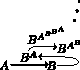
\includegraphics[width=0.4\textwidth]{fig/mrcatinf.pdf}
	\end{center}
\end{frame}

\begin{frame}[t]
\frametitle{$\times \dashv Hom$ adjunction}
\begin{block}{}
\abovedisplayskip=0pt
\begin{align*}
- \times B: \mathcal{C} & \rightleftarrows \mathcal{C}: (-)^B\\
\Mor_{\mathcal{C}}(B^{A^B} \times B, B^{A^B}) & \cong  \Mor_{\mathcal{C}}(B^{A^B}, B^{A^{B^B}})
\end{align*}
\end{block}
\begin{columns}[t]
    \begin{column}{0.5\textwidth}
\begin{block}{in components}
			$$
			\xymatrix{
			& B^{A^B} \times B \ar[d]^-{i \times 1_B} \ar[dl]_{\bar{i}} & B^{A^B} \ar@{.>}[d]^-{i}\\
			B^{A^B} & B^{A^{B^B}} \times B \ar[l]^{\epsilon} & B^{A^{B^B}}
			}
			$$
		\end{block}
    \end{column}
    \begin{column}{0.5\textwidth}
		\begin{block}{adjoint correspondence}
		\abovedisplayskip=0pt
		$$
			\frac{B^{A^B} \times B \longrightarrow B^{A^B}}{B^{A^B} \longrightarrow B^{A^{B^B}}}
		$$
		the counit is the evaluation map
		$$
			\epsilon = ev_{B^{A^B}} \colon B^{A^{B^B}} \times B \longrightarrow B^{A^B}
		$$
		\end{block}		
    \end{column}
\end{columns}
\end{frame}


\begin{frame}[t]
\frametitle{Exponentiation diagram}

$$
			\xymatrix{
			 LOL &LoL &Sublol \\
			  B^{A^{B^A}} \times A \ar[r]^{\epsilon} \ar[u]^{..^A} & B^{A^B} \ar[u]^{..} & B^{A^{B^B}} \times B\ar[l]^{\epsilon}\ar[u]^{..^B} \\
			 B^{A^A} \times A \ar[r]^{\epsilon} \ar[u]^{r^A} & B^A \ar[u]^{r} & B^{A^B} \times B\ar[l]^{\epsilon}\ar[u]^{r^B} \\
			B^A \times A \ar[r]^{\epsilon} \ar[u]^{g^A} & B \ar[u]^{g} & B^B \times B\ar[l]^{\epsilon}\ar[u]^{g^B} \\
			A^A \times A \ar[r]^{\epsilon} \ar[u]^{f^A} & 
			A\ar[u]^{f} & A^B\times B\ar[l]^{\epsilon}\ar[u]^{f^B} }
			$$

\end{frame}